%%%%% Beginning of preamble %%%%%
\documentclass[12pt]{article} 

%What kind of document (article) and what size
%Packages to load which give you useful commands
\usepackage{amssymb, amsmath, amsthm} 
\usepackage{epsfig,graphicx} 
\usepackage{caption}
\usepackage{subcaption}


%Sets the margins
\textwidth = 6.5 in 
\textheight = 9 in 
\oddsidemargin = 0.0 in 
\evensidemargin = 0.0 in 
\topmargin = 0.0 in 
\headheight = 0.0 in 
\headsep = 0.0 in \parskip = 0.2in \parindent = 0.0in

\begin{document} 

\section{Network and Dynamics}

\textbf{Put a blurb here about the distinction between `dynamics on vs dynamics of' with networks?}

First, we consider the most general case of a dynamics \emph{on} a \emph{structurally-static} network. We fix some notation, following \cite{kolaczyk2009statistical}. Let $G = (V, E)$ be the graph that represents the $|V|$ vertices in the network and the $|E|$ edges between them. We will consider a random field evolving in time on this network. That is, for a finite network, let $X(t, v)$ denote the random variable in some countable alphabet $\mathcal{X}_{v}$ associated with vertex $v$ at time $t$. Overall, $X(t, v)$ is a time-varying random field whose dynamics take place on $G$ and are effected by the topology of $G$. Thus, for fixed $t$, $X(t, \cdot)$ is a random vector and for fixed $v$, $X(\cdot, v)$ is a random field. We will occasionally refer to the random field at a fixed timepoint $t$ as $\mathbf{X}(t) = (X(t, v_{1}), \ldots, X(t, v_{|V|})).$

For the real world problem we consider in this paper, $G$ corresponds to an (explicit/structural) social network, and $X(t,v)$ corresponds to some observed behavior of an individual $v$ at time $t$. Since the empirical data consists of the tweeting behavior of users on Twitter, we will frequently fix $\mathcal{X}_{v} = \{0, 1\}$ with $X(t, v) = 1$ indicating that user $v$ tweeted at time instant $t$, and $X(t, v) = 0$ indicating that user $v$ did not tweet at time instant $t$.

\section{Edge Weighting using Dynamics}

\textbf{Put a brief rationale for why we use this approach. Or perhaps this goes in an introductory section where we argue for the need to determine communities based on dynamics?}

Let $X^{u} = X(\cdot, u).$ That is, in what follows we implicitly assume the stationarity of $X(t, v)$ with respect to time\footnote{If we do not assume stationarity, the statistics we compute have meaning but are no longer estimators for the parameters we describe. See~\cite{vu2009information}.}. Denoting the joint distribution of $(X^{u}, X^{v})$ as $p(x^{u}, x^{v})$ and the associated marginals as $p(x^{u})$ and $p(x^{v})$, we then define the mutual information between two individuals in the usual way~\cite{cover2012elements} as
\begin{align}
	I[X^{u}; X^{v}] &= E\left[\log_{2} \frac{p(X^{u}, X^{v})}{p(X^{u})p(X^{v})}\right]\\
	&= \sum_{x^{u} \in \mathcal{X}^{u}, x^{v} \in \mathcal{X}^{v}} p(x^{u}, x^{v}) \log_{2} \frac{p(x^{u}, x^{v})}{p(x^{u}) p(x^{v})}.
\end{align}
The mutual information is not generally bounded on a standard interval. To allow for standardized weightings, we follow~\cite{shalizi2007discovering} and normalize the mutual information, noting that
\begin{align}
	I[X^{u}; X^{v}] = H[X^{u}] - H[X^{u} | X^{v}] \leq H[X^{u}]
\end{align}
(by the non-negativity of $H[X^{u} | X^{v}]$), and equivalently
\begin{align}
	I[X^{u}; X^{v}] = H[X^{u}] - H[X^{u} | X^{v}] \leq H[X^{v}].
\end{align}
Overall, this implies that
\begin{align}
	I[X^{u}; X^{v}] \leq \min \left\{ H[X^{u}], H[X^{v}]\right\},
\end{align}
so dividing by $\min \left\{ H[X^{u}], H[X^{v}]\right\}$ gives the normalized mutual information
\begin{align}
	I^{*}[X^{u}; X^{v}] = \frac{I[X^{u}; X^{v}]}{\min \{ H[X^{u}], H[X^{v}]\}} \label{normalized-MI}
\end{align}
which lies between 0 and 1.

Of course, in an empirical study, we do not know the information theoretic quantities associated with any two users. Instead, we must infer them from an observed time series. To do so, we use the maximum likelihood estimates for all quantities~\cite{paninski2003estimation}. In the absence a parametric model (which we do not assume here), this amounts to using the plug-in estimator for $p(x^{u}, x^{v})$ in (\ref{normalized-MI}). Assuming we observe $\{ (X(t, u), X(t, v)) \}_{t = 1}^{T}$, the plug-in estimator for $p(x^{u}, x^{v})$ is simply
\begin{align}
	\hat{p}(x^{u}, x^{v}) = \frac{\#(X(t, u) = x^{u}, X(t, v) = x^{v})}{T},
\end{align}
the proportion of times we observe a particular behavior in both individuals out of all behaviors observed.

As observed in~\cite{paninski2003estimation}, all estimators for information theoretic quantities are biased, including the plug-in estimator. However, the bias is generally proportional to the size of the joint alphabet $\mathcal{X}^{u} \times \mathcal{X}^{v}$ and inversely proportional to the sample size $T$. Since we will typically take $\mathcal{X}^{u} = \{0, 1\}$ for all individuals $u$, $|\mathcal{X}^{u} \times \mathcal{X}^{v}| = 4$, and the bias will be small for the sample sizes we consider.

\textbf{How this gets used in a community detection algorithms goes here (or in a nearby section).}

\section{Examples}

We apply the methodology developed above to two cases: a toy model of user dynamics and a real world dataset from Twitter.

\subsection{Coupled Bernoulli Processes Embedded in a Structural Network Drawn from a Stochastic Block Model}

\textbf{Describe the toy model in generalities.}

\subsubsection{Stochastic Block Model}

\label{Sec-SBM}

We use the stochastic block model~\cite{holland1983stochastic} as a generative model for the structural network. The basic stochastic block model is a popular model for simple community structure. We will specify the community of a user $u$ by $C(u)$ and the set of all communities by $\mathcal{C}$. Each individual $u$ in the network is assigned to a (latent) community $C(u) = c \in \mathcal{C}$. Edges are then placed between each user $u$ and $v$ with probability $p_{uv} = p_{C(u), C(v)}$ depending only on the membership the two users. Typically, for assortative communities, $p_{cc} > p_{cc'}$ for all $c \neq c' \in \mathcal{C}$. That is, the density of links within a community is greater than the density of links between communities, which is the standard definition of community structure. These edge probabilities can be collected into a matrix $\mathbf{P}$ where $(\mathbf{P})_{cc'} = p_{cc'}.$ If we fix $p_{cc} = p_{\text{in}}$ and $p_{cc'} = p_{\text{out}}$ for all $c \neq c' \in \mathcal{C}$, we obtain an edge probability matrix like Figure~\ref{Fig-SBM}. This clearly posses a `block' structure (hence the name stochastic block model) with clear communities. The adjacency matrix for a particular realization from this model resembles Figure~\ref{Fig-SBM_Realization}.

\begin{figure}[h!]
  \centering
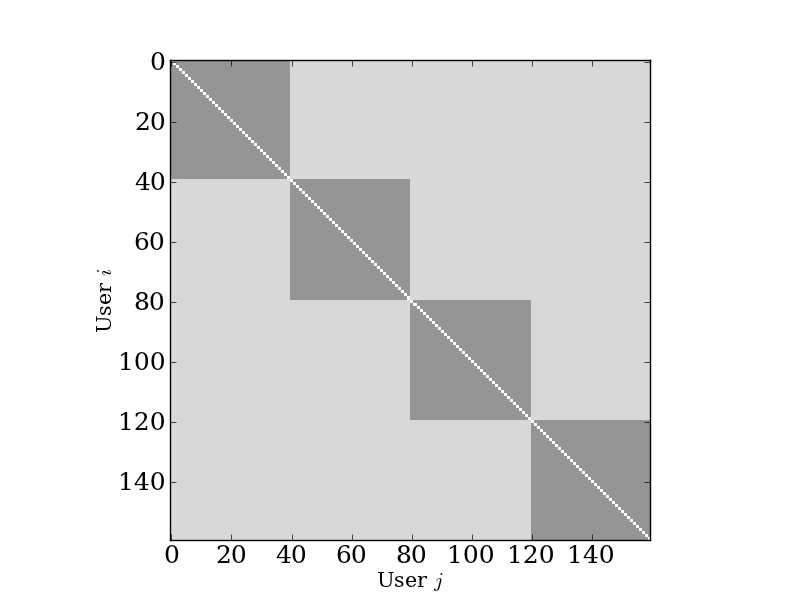
\includegraphics[width=0.75\textwidth]{Figures/prob_mat.png}
\caption{The edge probability matrix \textbf{P} for a stochastic block model with four communities each with 40 members.}
\label{Fig-SBM}
\end{figure}

\begin{figure}[h!]
  \centering
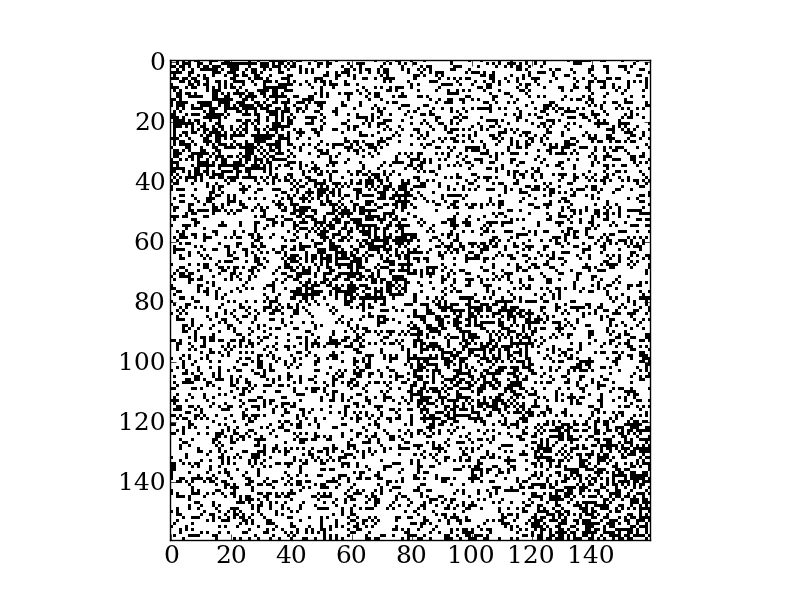
\includegraphics[width=0.75\textwidth]{Figures/adj_mat.png}
\caption{The (undirected) adjacency matrix $\mathbf{A}$ from a realization of the stochastic block model specified by the edge probability matrix \textbf{P} from Figure~\ref{Fig-SBM}.}
\label{Fig-SBM_Realization}
\end{figure}

\subsubsection{Coupled Bernoulli Process}

Previous work~\cite{ver2012information} has considered modeling users on Twitter as coupled Poisson processes. In this model, the users are embedded in a directed network, with each vertex in the graph corresponding to a user and each directed edge indicating the presence of `influence' of the initiating user on the terminal user. Influence was modeled as follows: after a user $u$ tweets, the user exerts an influence on its directed neighbors by increasing the instantaneous rate of their associated Poisson process for some interval of time. The authors of~\cite{ver2012information} took the coupling term to decay as a reciprocal power of the time since the tweet occurred.

In this work, we consider a modified version of this model. (\textbf{Mention connections to (directed) Susceptible-Infected-Susceptible type models?}) First, since communication on digital social networks such as Twitter occur in discrete time, we explicitly model each user as a \emph{Bernoulli} process, the discrete-time analog of a Poisson process. Second, in this initial work, we only consider an influence to occur over a single time delay. This corresponds to a choice of time scale. Thus, at a given time instant $t$, the probability of a particular user tweeting, given the entire past behavior of all of the users is
\begin{align}
	P(X(t, v) = 1 | \mathbf{X}(t-1), \mathbf{X}(t-2), \ldots) &= P(X(t,v) = 1 | \{ X(t-1, u) : u \in \mathcal{N}(v)\})\\
	&=\min \left\{p_{v} + \sum_{u \in \mathcal{N}(v)} \iota_{uv} 1[X(t-1, u) = 1], 1\right\} \label{Eq-Bernoulli_Model}
\end{align}
where $\mathcal{N}(v)$ denotes the directed neighbors of $v$ (those users in the network with directed edges from themselves to $v$), and $\iota_{uv}$ denotes the influence of user $u$ on user $v$.

\begin{figure}[h!]
  \centering
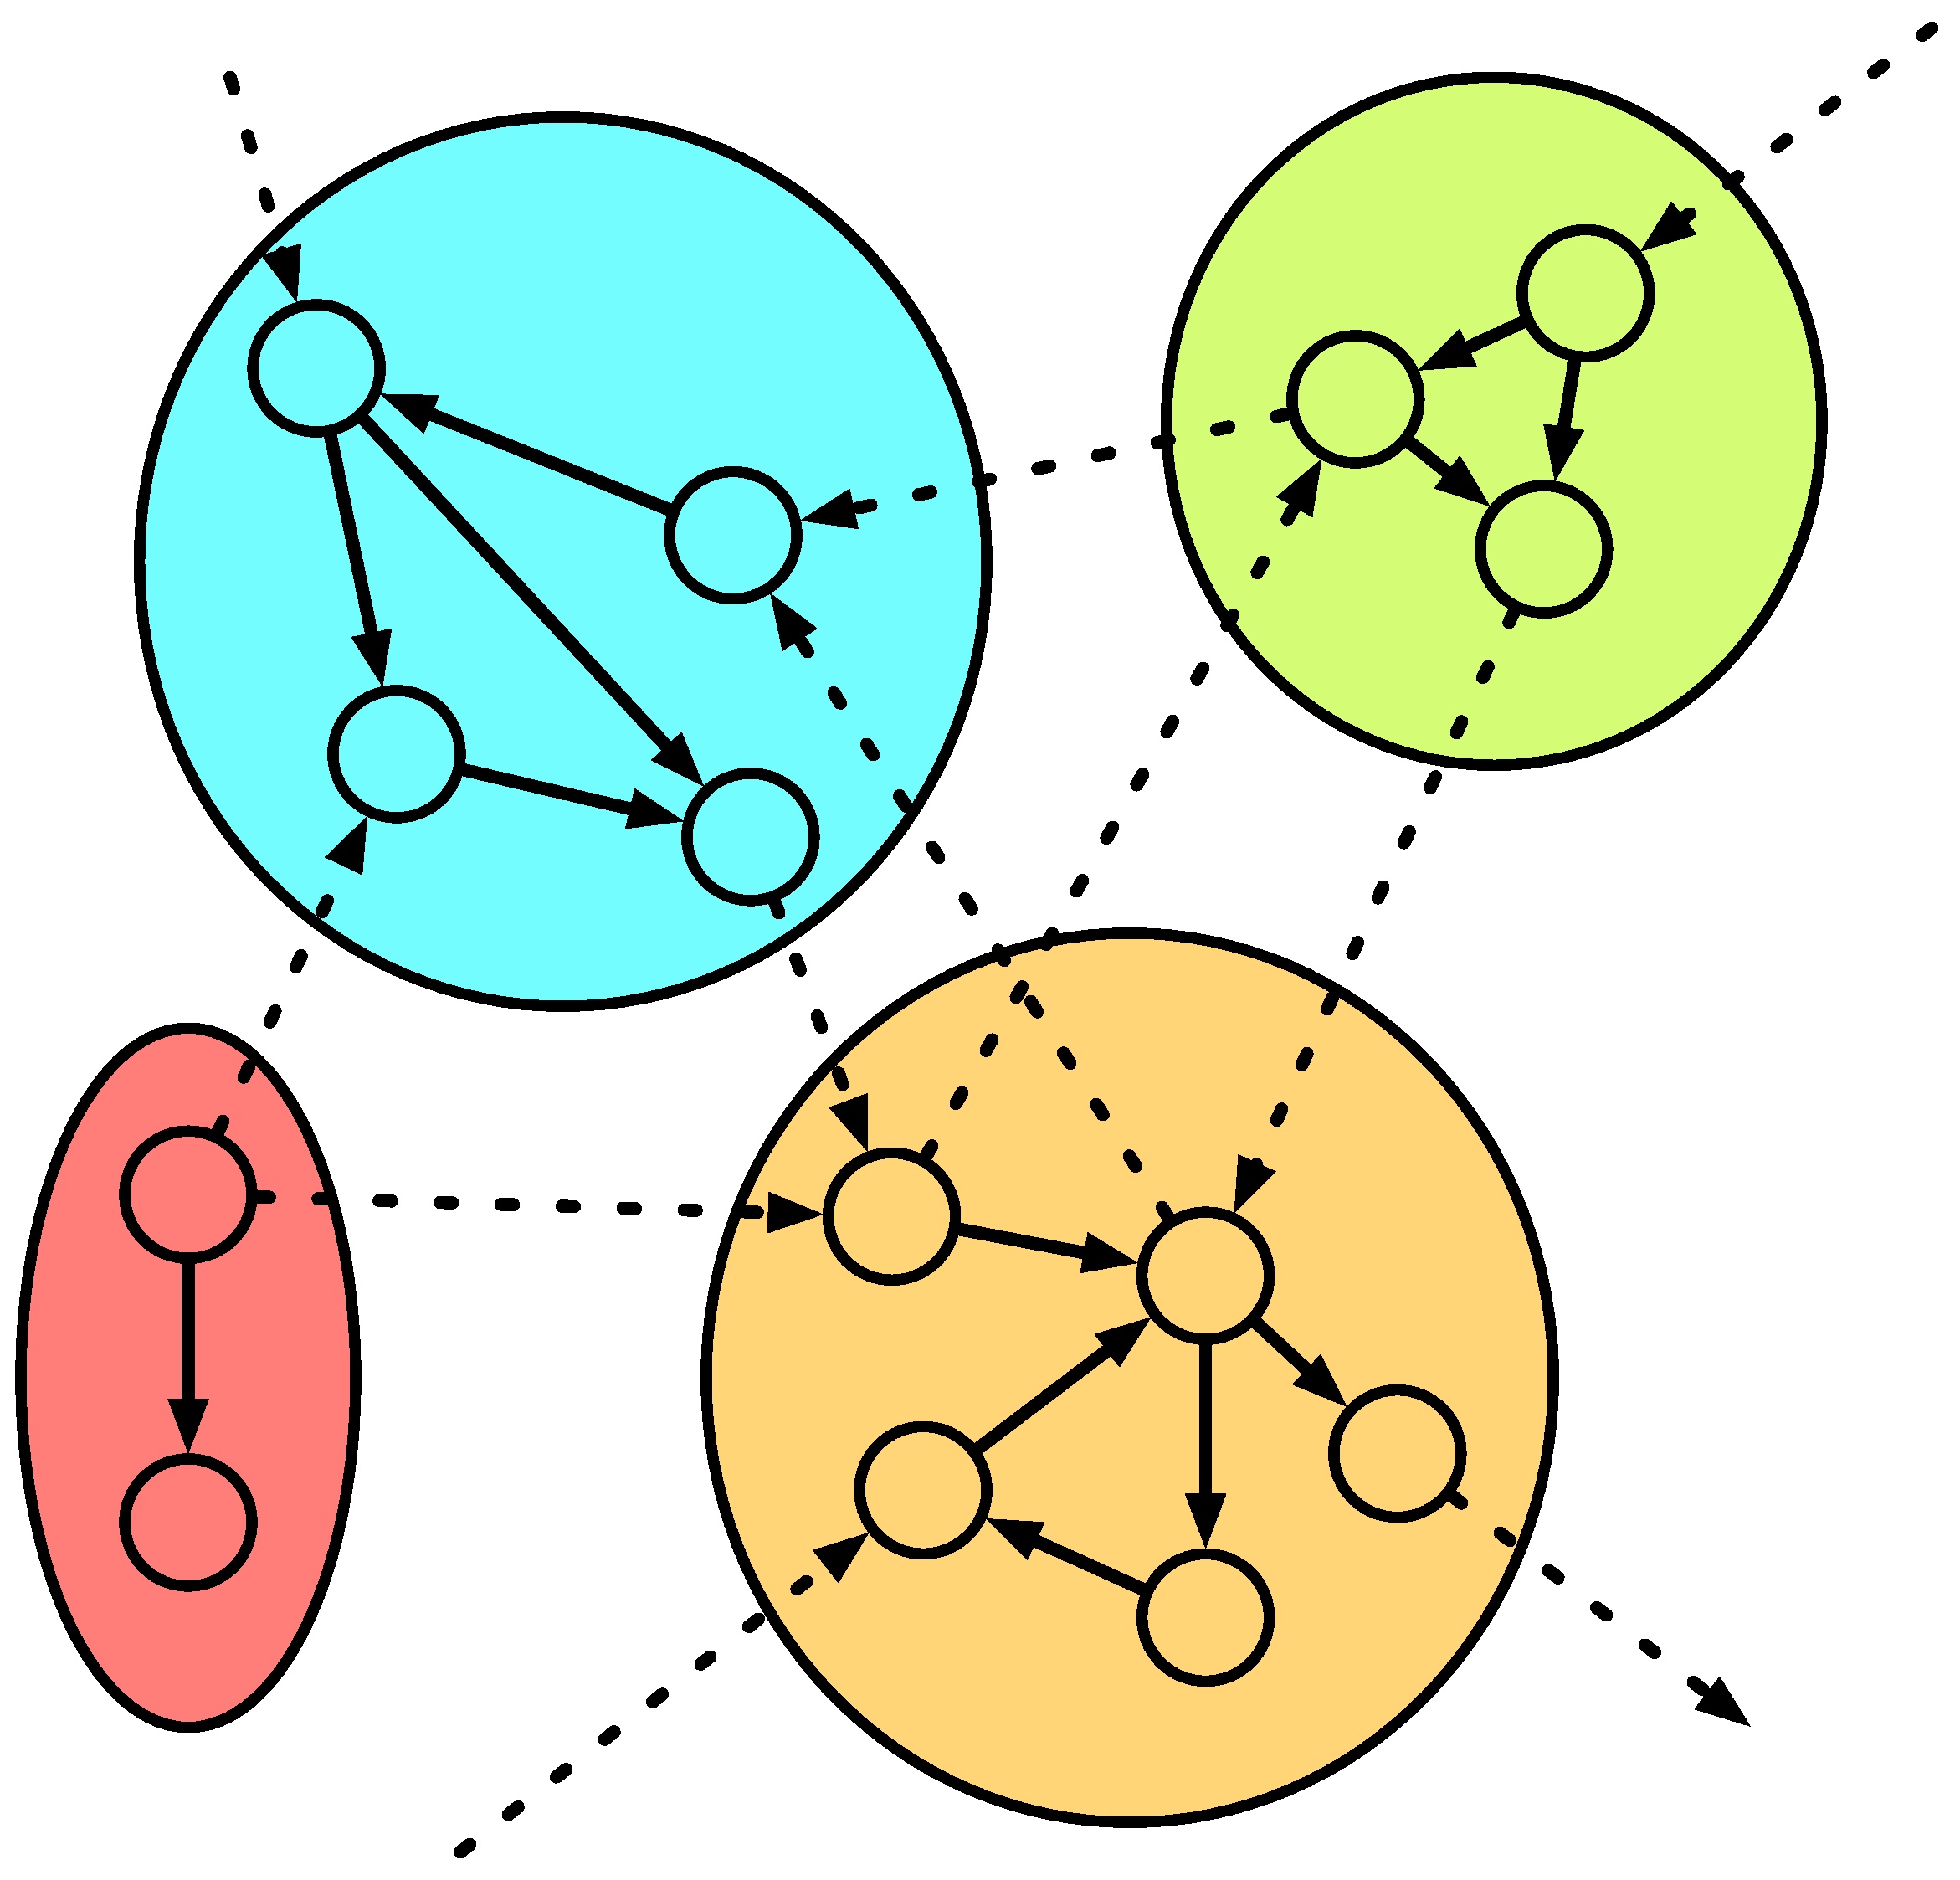
\includegraphics[width=0.3\textwidth]{Figures/Communities.eps} \hspace{1 in}
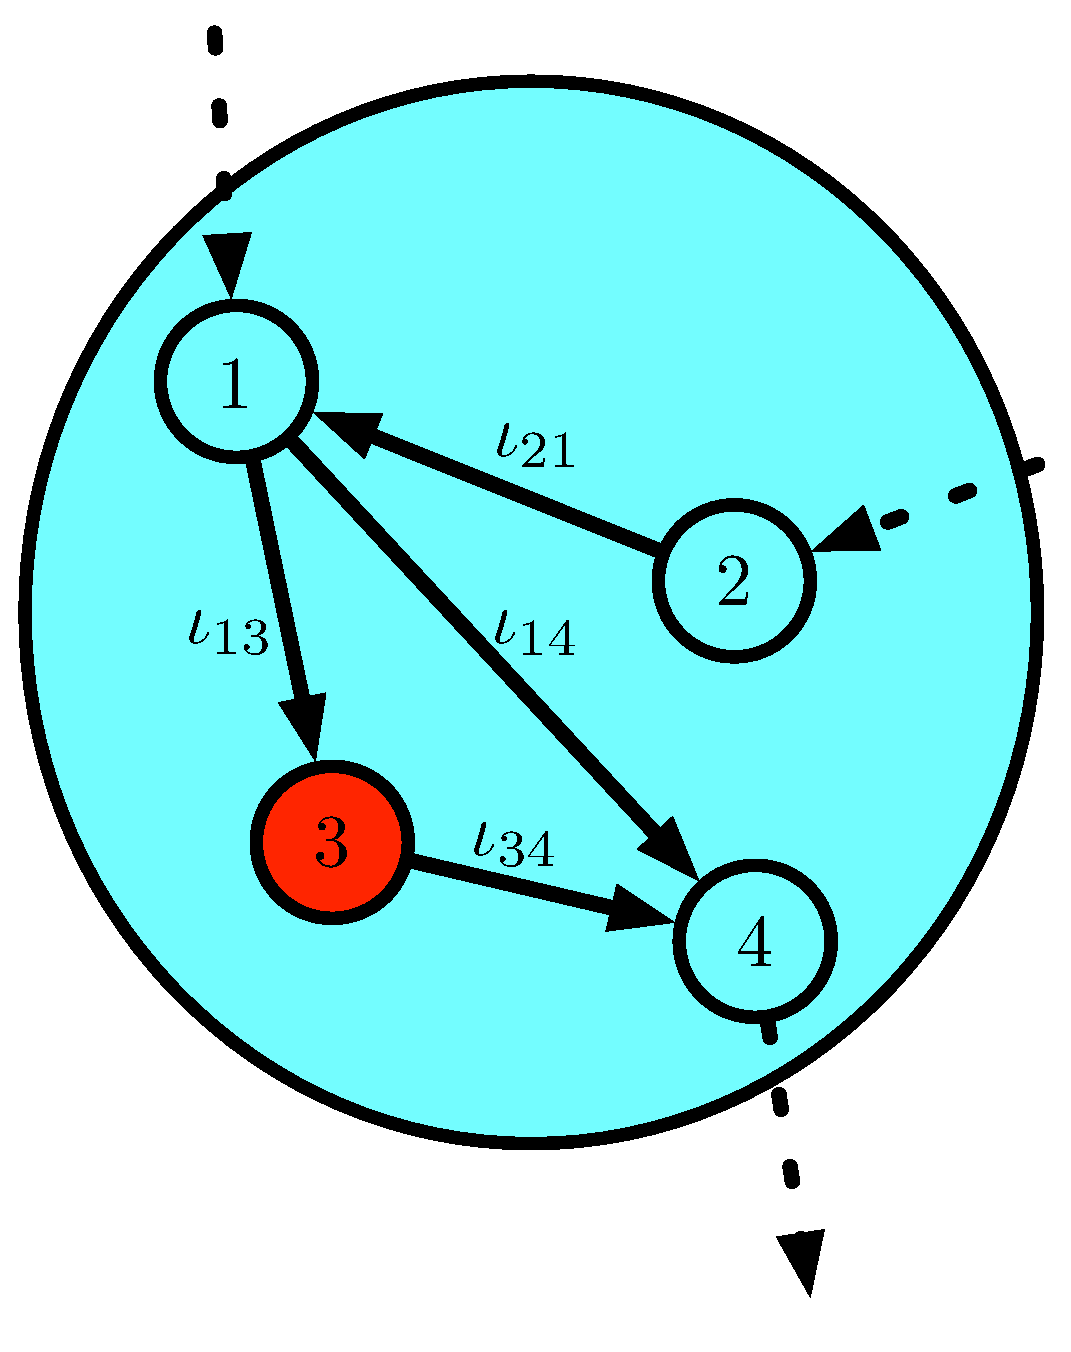
\includegraphics[width=0.3\textwidth]{Figures/Toy2.eps}
\caption{Schematics for the coupled Bernoulli model. Left: A collection of communities defined by the dynamics of their users. Right: Focusing on the influencers of a particular user.}
\label{Fig-Toy_Bernoulli}
\end{figure}

A schematic for this model is shown in Figure~\ref{Fig-Toy_Bernoulli}. In the left schematic, each solid circle corresponds to a set of nodes in a particular dynamical / functional (\textbf{whatever word we decide to use}) community. Note that these communities may differ from the \emph{structural communities} as defined by the stochastic block model in Section \ref{Sec-SBM}. In particular, we will take $\iota_{uv}$ to be larger between two nodes $u$ and $v$ within the dynamical community than between two nodes in different dynamical communities. In the right schematic, we focus on user 3. For this user, we see that the equation determining the probability of that user tweeting at time $t$ (Equation (\ref{Eq-Bernoulli_Model})) reduces to
\begin{align}
	P(X(t, 3) = 1 | \mathbf{X}(t-1), \ldots) &= P(X(t,3) = 1 | X(t, 1)) \\
		&= \min \left\{p_{3} + \iota_{13} 1[X(t-1, 1) = 1], 1\right\}\\
		&= \text{base rate } + \text{ influence,}
\end{align}
a base probability plus the influence of 3's directed neighbors.

\subsubsection{Choice of Parameters for Toy Model}

For the results presented in this paper, we took $p_{\text{in}} = p_{\text{out}} = p = \ldots$ (\textbf{not in the code... but I can figure it out from the sampled adjacency matrix}). Thus, any `structural' communities are spurious. For each edge generated by the stochastic block model, the direction of the edge was chosen at random. We took $\iota_{\text{in}} = \frac{0.7}{4}$ and $\iota_{\text{out}} = \frac{0.07}{4}$. Thus, the influence of users within a dynamical community is ten times the influence of users outside the dynamical community. The value for $\iota_{\text{in}}$ was chosen to be below a critical value $\iota^{*}_{\text{in}}$ (dependent on $p$) that lead the users in each community to constantly tweet.

\subsection{Twitter Dataset}

The data consists of the Twitter statuses of 12,043 users over a 49 day period. The users are embedded in a 15,000 node network collected by performing a breadth-first expansion from a seed user. Once the seed user was chosen, the network was expanded to include his/her followers, only including users considered to be active (users who tweeted at least once per day over the past one hundred tweets). Network collection continued in this fashion by considering the active followers of the active followers of the seed, etc.

The statuses of each user were transformed into a binary time series using their time stamp as follows. For each user $u$, we consider only the relative times of their tweets with respect to a reference time. Denote these times by $\{ \tau^{u}_{j}\}_{j = 1}^{n_{u}}$. Let the reference start time be $t_{0}$ and the coarsening amount be $\Delta t$. From the tweet times, we can generate a binary time series $\{ X(i, u)\}_{i = 1}^{T}$, where
\begin{align}
	X(i, u) = \left\{ \begin{array}{cl}
		1 &: \text{$ \exists \tau^{u}_{j} \in [t_{0} + (i - 1) \Delta t, t_{0} + i \Delta t)$} \\
		0 &: \text{ otherwise}
	\end{array}\right. .
\end{align}
In words, $X(i, u)$ is 1 if user $u$ tweeted at least once in the time interval $[t_{0} + (i - 1) \Delta t, t_{0} + i \Delta t)$, and 0 otherwise. Because the recorded time of tweets is restricted to a 1-second resolution, a natural choice for $\Delta t$ is 1 second. However, computing mutual information between second-resolution tweet series would neglect medium- to long-range influences between individuals. Thus, we generally take $\Delta t$ to be on the order of minutes.

In this paper, only tweets made between 7 AM and 10 PM (EST) were considered. For any second during this time window, a user either tweets, or does not. Thus, each day can be considered as a binary time series of length 57,600, with a 1 at a timepoint if the user tweets, and a 0 otherwise.

\bibliographystyle{plain}
\bibliography{../references}

\end{document}